\documentclass[12pt]{article}
\usepackage[utf8]{inputenc}
\usepackage[english]{babel}
\usepackage[letterpaper, portrait, margin=1in]{geometry}
\usepackage{amsmath}
\numberwithin{equation}{section}
\usepackage{amssymb}
\usepackage{graphicx}
\usepackage{parskip}
\usepackage{xcolor}
\usepackage{physics}
\usepackage{empheq}
\usepackage{cancel}
\usepackage{hyperref}
\hypersetup{colorlinks = true, urlcolor = blue, linkcolor = red, citecolor = red}
\usepackage{enumerate}
\usepackage{tikz}
\usepackage{float}
\usepackage{tcolorbox}
\usepackage{booktabs}
\usepackage[bottom]{footmisc}

% Default fixed font does not support bold face
\DeclareFixedFont{\ttb}{T1}{txtt}{bx}{n}{12} % for bold
\DeclareFixedFont{\ttm}{T1}{txtt}{m}{n}{12}  % for normal

% Custom colors
\usepackage{color}
\definecolor{deepblue}{rgb}{0,0,0.5}
\definecolor{deepred}{rgb}{0.6,0,0}
\definecolor{deepgreen}{rgb}{0,0.5,0}

\usepackage{listings}

% Python style for highlighting
\newcommand\pythonstyle{\lstset{
language=Python,
basicstyle=\ttm,
morekeywords={self},              % Add keywords here
commentstyle=\color{gray},
keywordstyle=\ttb\color{deepblue},
emph={MyClass,__init__},          % Custom highlighting
emphstyle=\ttb\color{deepred},    % Custom highlighting style
stringstyle=\color{deepgreen},                        % Any extra options here
showstringspaces=false
}}


% Python environment
\lstnewenvironment{python}[1][]
{
\pythonstyle
\lstset{#1}
}
{}

% Python for external files
\newcommand\pythonexternal[2][]{{
\pythonstyle
\lstinputlisting[#1]{#2}}}

% Python for inline
\newcommand\pythoninline[1]{{\pythonstyle\lstinline!#1!}}

\usepackage{xcolor}
\usepackage{fancyhdr}
\pagestyle{fancy}
\fancyhf{}
\fancyfoot[C]{\color{lightgray} Python Lecture III Notes}
\fancyfoot[L]{\color{lightgray} \today}
\fancyfoot[R]{Page \thepage}
\renewcommand{\headrulewidth}{0pt}
\renewcommand{\footrulewidth}{0pt}
\begin{document}

\section{Review}

\textbf{Last time:}
\begin{itemize}
    \item Last week's HW was using Jupyter notebook. Any questions on Jupyter?
    \item Basic Python types and operations.
    \item Conditionals
\end{itemize}

\section{Conditionals Example}
\textbf{Fizz Buzz!} You are given a number \verb|num|. Your program should:
\begin{enumerate}
    \item Print `fizz' if divisible by 3
    \item Print `buzz' if divisible by 3
    \item Print `fizzbuzz' if divisible by 3 and 5
    \item Print the number otherwise
\end{enumerate}

\begin{python}
num = 15 # some number
d3 = (num%3)==0
d5 = (num%5)==0
if d3 and d5:
    print('fizzbuzz')
elif d3:
    print('fizz')
elif d5:
    print('buzz')
else:
    print(num)
\end{python}

\section{Loops}
\begin{itemize}
    \item We often want to run a piece of code many times
    \item While and for loops
\end{itemize}

\textbf{While loop}: runs WHILE a condition true
\begin{python}
import random as rand
num = 0
while num!=5:
    print('The number is ' + str(num))
    num = rand.randint(1,10) # random integer between 1-10

print('The number is 5!')
\end{python}

\textbf{For loop:} iterates through a type of object called ITERABLE. There are two types of iterable objects that we're concerned with,
\begin{enumerate}
    \item range(a, b) = $\{x : a\leq x <b\}$
    \item range(b) = $\{0 : a\leq x <b\}$
    \item lists
\end{enumerate}

\begin{python}
# prints 1, 2, ..., 10
for i in range(1,11):
    print(i)

# prints contents of the list
lst = [3, 1, 4, 1, 5]
for i in lst:
    print(i)
    
# double the contents of a list
for i in range(len(lst)):
    lst[i] = lst[i]*2 
\end{python}

\section{Functions}
\begin{itemize}
    \item Perform a repetitive task that reacts to some input and has some output
    \item Functions are black boxes. Someone can hand you a function they wrote and you don't have to understand HOW it works but only WHAT it does.
    \begin{figure}[H]
	    \centering
	    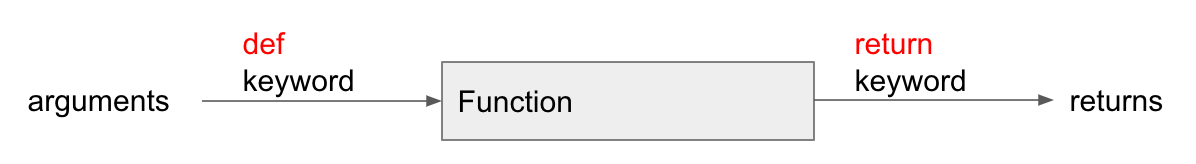
\includegraphics[width=12cm] {box}
    \end{figure}
    \item The name of a function is always followed by \verb|()|
    \item Defining a function: 
    \begin{python}
    def say_hi():
        print('hi!')
    \end{python}
    \item Calling a function:
    \begin{python}
    >>> say_hi()
    hi!
    \end{python}
    \item Functions can take arguments: information that you pass to the code inside the function.
    \begin{python}
    def greet(name):
        print('Hi {}, how are you today?'.format(name))
        
    >>> greet('James')
	Hi James, how are you today?
    \end{python}
    \item Function can return arguments:
    \begin{python}
    def add(x, y):
        sum = x+y
        return sum
        
    >>> result = add(1, 2)
    >>> print(result)
    3
    \end{python}
    \item Notice that the order of your arguments matters!
    \item If no return statement if provided, Python returns None by default
    \item Default arguments: you can specify that an argument should have a default value if not provided by the user.
    \begin{python}
    def get_harmonic(freq, harmonic=2):
        return freq*harmonic
    
    >>> get_harmonic(100) #200
    >>> get_harmonic(100, 3) #300
    >>> get_harmonic(100, harmonic=3) #300, more explicit
    \end{python}
    \item Unpacking an iterable: taking an iterable object (e.g. list) and unpacking it's contents.
    \begin{python}
    >>> lst = [1, 2]
    >>> add(lst[0], lst[1])
    3
    >>> add(*lst)
    3
    >>> print(*lst)
    1 2
    \end{python}
    \item Packing an iterable: what if you want to write a function that takes an unspecified number of arguments?
    \begin{python}
    def add(*args):
        sum = 0
        for n in args:
            sum = sum + args
        return sum
    
    >>> add(1, 2, 3)
    6
    >>> add(*lst)
    3
    \end{python}
\end{itemize}

\textbf{Demo: finding all primes up to 1000}
\begin{itemize}
    \item We only need to check factors up to $\lfloor n/2 \rfloor$. Proof: if $x\cdot y = n$ , then $y = n/x \leq 2$, which we have already checked.
\end{itemize}

\begin{python}
def is_prime(n):
    for i in range(2, int(n/2)):
        if n%i==0:
            return False
    return True

primes = []
for n in range(1, 10001):
    if is_prime(n):
        primes.append(n)

print(*primes, sep=',')
\end{python}

\section{Errors}
There are can be many sources of error in your code:
\begin{itemize}
    \item syntax
    \item runtime errors
\end{itemize}
Whenever an error arises \textbf{and is not handled by your code}, your program terminates and a stack trace is initiated.

\begin{python}
1 # returns if n is divisible by x
2 def is_divisible(n, x):
3 	return n%x == 0
4 
5 print(is_divisible(1,0))

>>> python Demo.py
Traceback (most recent call last):
  File "demo.py", line 1, in <module>
  File "demo.py", line 2, in f
ZeroDivisionError: integer division or modulo by zero
\end{python}

\textbf{Traceback:}
\begin{itemize}
    \item The traceback traces back the sources of the error
    \item Read the traceback from bottom to top
    \item Bottom line: What error caused the code to stop and any messages that accompany the error. 
    \item Moving bottom to top, the most recent line of code where the error occurred.
    \item Read the traceback to effectively debug code!!
\end{itemize}

\textbf{Catching exceptions}: sometimes, when an error occurs, you want your code to move on.
\begin{python}
try:
    print(is_divisible(1,0))
except ZeroDivisionError:
    print('There was a zero division error!')

print(is_divisible(3,2))

>>> python Demo.py
There was a zero division error! 
False
\end{python}
\begin{itemize}
    \item to handle any error, catch \verb|Exceptions|
\end{itemize}

\textbf{Raising exceptions: }
\begin{itemize}
    \item Sometimes, you want your code to cause exceptions.
sometimes, you want your code to cause exceptions.
    \item E.g. want to make sure that the arguments that the user passes to your function make sense
    \item You can cause an error with the \verb|raise| keyword
    \item Assertion error: assert that a condition is true, otherwise an \verb|AssertionError| is thrown.
\end{itemize}
\begin{python}
def dogs(name):
    if type(name) != str:
        raise TypeError("Dog's name is not a string.")
    
    assert len(name)>0, "Name your dog, you bastard!"
    
    print("Your dog's name is " + name)
\end{python}

\section{Next Week}
\begin{itemize}
    \item A miscellany of topics
    \item List comprehensions, dictionaries, lambda functions, importing, pip
\end{itemize}

\end{document}
